\section{Gravitational-Wave signals from binary neutron star mergers}
\textcolor{blue}{Explain the use for this section.}\\
Gravitational waves from two inspiraling neutron stars are among the most interesting signals gravitational wave detectors can detect. They convey information about the highly relativistic regimes of gravity, about the structure of the component stars and about the formation channels of black holes or heavy neutron stars. \textcolor{red}{[Citations]} They are however also very hard to detect, as binary neutron star (\gls{bns}) systems are very light systems, when compared to inspiraling binary black holes (\gls{bbh}).\\
Part 1 of this section will discuss how gravitational waves (\gls{gw}) are formed and what influences the structure of the resulting waveforms. Part 2 will go over the current method of detecting \gls{gw} and discuss the advantages and drawbacks. \textcolor{red}{Need to specify, that I use Einstein sum convention in this section and that latin indices are spacial indices, whereas greek indices are over all four components.}
\subsection{The waveform}
\textcolor{blue}{Explain how the waveform looks like, what it depends on, maybe give the concept how it works in the context of linearized theory (quote bachelor thesis), cite important papers regarding the waveform theory.}\\
Gravitational waves are a solution to the Einstein-equation
\begin{equation}\label{def:einstein_equation}
\mathcal{G}_\mn = \frac{8\pi G}{c^4}T_\mn,
\end{equation}
where $\mathcal{G}_\mn$ is the Einstein-tensor, $T_\mn$ is the energy-momentum-tensor, $G$ is the gravitational constant and $c$ is the speed of light in vacuum. They can be derived in their linear form, by setting assuming the metric to be a linear correction to the flat metric $\eta_\mn$
\begin{equation}
g_\mn = \eta_\mn + h_\mn.
\end{equation}
With this approximation the Einstein-equation \eqref{def:einstein_equation} simplifies to
\begin{equation}\label{def:einstein_linear}
\mathcal{G}_\mn=\frac{1}{2}\lr{\partial_{\alpha\mu}h^\alpha_\nu+\partial^\alpha_\nu h_{\mu\alpha} - \partial_\mn h- \Box h_\mn - \eta_\mn\Box h} = \frac{8\pi G}{c^4}T_\mn,
\end{equation}
where $h\coloneqq\eta^\mn h_\mn$ and $\Box\coloneqq\eta^\mn\partial_\mn$.\\
This equation has $10$ independent components, of which only $2$ are physical. To reduce the number of independent components, one can choose gauge conditions through the coordinate transformation ${x'}^\mu=x^\mu+\xi^\mu$, which leaves the Einstein equation invariant. One of these gauge conditions is the DeDonder gauge
\begin{equation}
\partial^\alpha \bar{h}_{\alpha\mu} = 0,
\end{equation}
where $\bar{h}_\mn\coloneqq h_\mn - \frac{1}{2}\eta_\mn h$. It can be realized by choosing $\Box\xi_\mu =\partial^\alpha \bar{h}_{\alpha\mu}$. In this gauge the linearized Einstein equation \eqref{def:einstein_linear} reduces to
\begin{equation}\label{def:gw_equation}
\Box\bar{h}_\mn=-\frac{16\pi G}{c^4}T_\mn.
\end{equation}
This gauge however leaves another freedom, as another transformation ${x'}^\mu=x^\mu+\xi^\mu$ could be applied, when $\Box\xi_\mu =0$. This can be used, such that the gauge to also satisfy $\bar{h}=-h=0$ and $\bar{h}_{0\mu} = 0 = \bar{h}_{3\mu}$. The gauge is named transverse-traceless-gauge (\gls{tt}) and results in the metric to be of the form
\begin{equation}\label{def:tt_gauge}
h_\mn^\text{\gls{tt}}=
\begin{pmatrix}
	0 & 0         & 0        & 0\\
	0 & h_+       & h_\times & 0\\
	0 & -h_\times & h_+      & 0\\
	0 & 0         & 0        & 0\\
\end{pmatrix}.
\end{equation}
\eqref{def:tt_gauge} now has only the two independent components $h_+$ and $h_\times$ left, which are called the ''plus-'' and ''cross-polarization'' of a \gls{gw}.\medskip\\
Evaluating \eqref{def:gw_equation} in vacuum reveals the wave-like character of $h_\mn$, as
\begin{equation}\label{def:gw_wave_equation}
\Box\bar{h}_\mn =0
\end{equation}
is a wave equation. Its solutions travel at the speed of light. Therefore \gls{gw} travel through space-time at the speed of light. The effect a solution of this equation has on a ring of resting test masses is shown in \autoref{fig:gw_test_masses}. (chapter 3 \cite{bachelor})\medskip\\
\begin{figure}
\centering
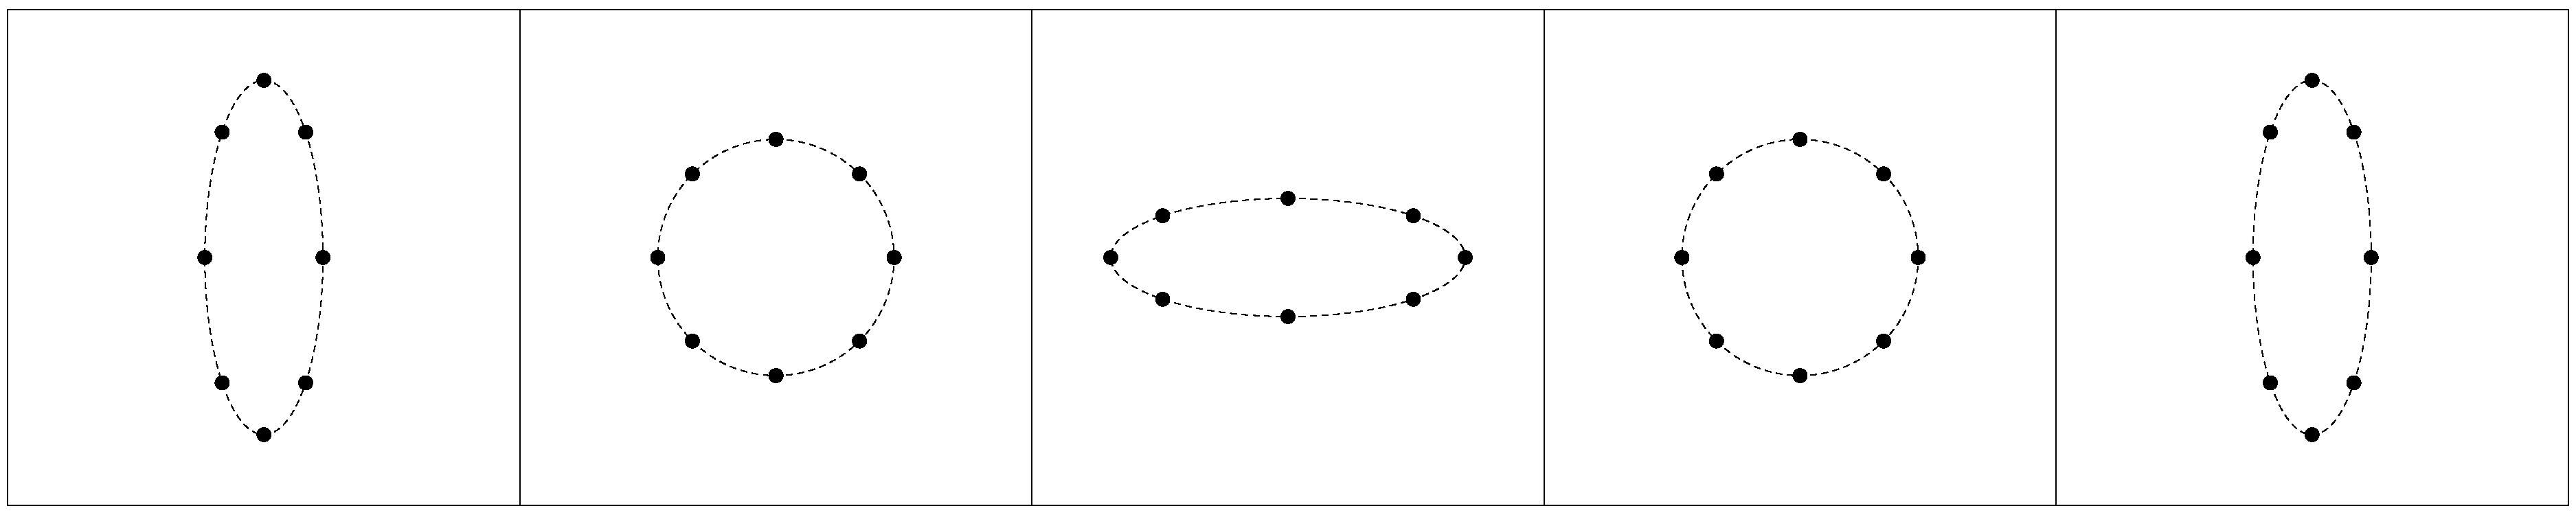
\includegraphics[width=\textwidth]{effect_gw.pdf}
\caption[Effect of GW on ring of test masses]{This image is taken from \cite{bachelor}. It shows the effect of a \gls{gw} passing orthogonaly through a ring of test masses.}\label{fig:gw_test_masses}
\end{figure}
\eqref{def:gw_wave_equation} shows, that \gls{gw} exist and can travel through space. It does however not specify how these waves are produced. To do so, the energy-momentum-tensor cannot be set to $0$. Instead the full equation \eqref{def:gw_equation} needs to be solved. The solution is known to be
\begin{equation}
\bar{h}\lr{t, \vec{x}}=\frac{4 G}{c^4}\int\Diff{3}x'\ \frac{T_\mn\lr{t-\frac{\norm{\vec{x}-\vec{x}'}}{c},\vec{x}'}}{\norm{\vec{x}-\vec{x}'}}.
\end{equation}
For simplification it is assumed, that the observer is far from the source when compared to the size of the support of $T_\mn$, such that $\norm{\vec{x}-\vec{x}'}\approx r\coloneqq\norm{\vec{x}}$. Therefore we need to solve
\begin{equation}
\bar{h}\lr{t, \vec{x}}=\frac{4 G}{c^4}\frac{1}{r}\int\Diff{3}x'\ T_\mn\lr{t-\frac{r}{c},\vec{x}'}.
\end{equation}
This equation can be solved to yield
\begin{equation}
h_{ab}^\text{\gls{tt}}\lr{t,\vec{x}}=\frac{2 G}{c^4}\frac{1}{r}\ddot{I}_{ab}^\text{\gls{tt}}\lr{t-r/c},
\end{equation}
where $\ddot{I}_{ab}^\text{\gls{tt}}$ is the transverse-traceless-projection of the second time derivative of the second mass moment
\begin{equation}\label{def:quad_st_1}
\ddot{I}^{ab}=c^2\partial_0^2 \int\Diff{3}x'\ x'^a x'^b T^{00} = 2\int\Diff{3}x'\ T^{ab}.
\end{equation}
As the quadrupole moment is simply the traceless second mass moment and we project it to its traceless part anyways, \eqref{def:quad_st_1} can be rewritten as
\begin{equation}
\boxed{h^{\gls{tt}}_{ab}\lr{t,\vec{x}} = \frac{2 G}{c^4}\frac{1}{r}\ddot{Q}^{\gls{tt}}_{ab}\lr{t-r/c},}
\end{equation}
with $Q_{ab}\coloneqq I_{ab} - \frac{1}{3}\delta_{ab}I^c_c$. This is the famous quadrupole formula. (chapter 5.2 in \cite{bachelor})\medskip\\

\noindent To calculate the \gls{gw} a binary system outputs, $I_{ab}$ or $Q_{ab}$ needs to be specified. Furthermore the transverse-traceless-projection needs to be calculated. The projection turns out to be ((3.64) in \cite{gwv1})
\begin{equation}
\ddot{I}_{ab}^\text{\gls{tt}}=
\begin{pmatrix}
\lr{\ddot{I}_{11}-\ddot{I}_{22}}/2 & \ddot{I}_{12}                     & 0\\
\ddot{I}_{21}                      & -\lr{\ddot{I}_{11}-\ddot{I}_{22}}/2 & 0\\
0                                  & 0                                 & 0
\end{pmatrix}_{ab}.
\end{equation}

\subsection{Matched filtering}
\textcolor{blue}{Explain what matched filtering is, why it works and how it is applied currently.}